\documentclass[aspectratio=169, 10pt]{beamer}

\usepackage{bm} % bold math
\usepackage{fontspec}
\usepackage{minted}
\usepackage{pgf-pie}
\usepackage{tikz}

% Custom commands and environments
\makeatletter
\newcommand\version[1]{\renewcommand\@version{#1}}
\newcommand\@version{}
\def\insertversion{\@version}

\newcommand\course[1]{\renewcommand\@course{#1}}
\newcommand\@course{}
\def\insertcourse{\@course}

\newcommand\coursetitle[1]{\renewcommand\@coursetitle{#1}}
\newcommand\@coursetitle{}
\def\insertcoursetitle{\@coursetitle}

\newcommand\lecturenumber[1]{\renewcommand\@lecturenumber{#1}}
\newcommand\@lecturenumber{}
\def\insertlecturenumber{\@lecturenumber}
\makeatother

\newcommand{\slidetitle}[1]{{\xbseries \large \structure{#1}} \bigskip}
\newcommand{\term}[1]{{\color{blue} #1}}
\newcommand{\leftspace}{\hspace{1em}}
\newcommand{\inlinearrow}{
  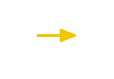
\begin{tikzpicture}[baseline]
    \node [anchor=base] (x) {};
    \draw [rawarrow] (x.mid west) -- ($(x.mid west) + (2em,0)$);
  \end{tikzpicture}
}

\newenvironment{slide}
{\begin{frame}[fragile,environment=slide]\vskip0pt plus 1filll}
{\vskip0pt plus 1filll\end{frame}}

% LaTeX

\setlength{\leftmargini}{1em}

% Common Information

\author{Jon Eyolfson}
\course{ECE 353}
\coursetitle{Systems Software}
\date{2024 Winter}

% fontspec

\defaultfontfeatures{Ligatures=TeX}
% \setmainfont{Domine}
\setsansfont{Inter}[
  FontFace={ul}{n}{Font=*-Thin},
  FontFace={el}{n}{Font=*-ExtraLight},
  FontFace={l}{n}{Font=*-Light},
  FontFace={sb}{n}{Font=*-SemiBold},
  FontFace={eb}{n}{Font=*-ExtraBold},
  FontFace={xb}{n}{Font=*-Black},
]
\setmonofont[Contextuals=AlternateOff, Ligatures=TeXOff]{Iosevka}[
  FontFace={xb}{n}{Font=*-Heavy},
]

%% Font Weights

\DeclareRobustCommand{\ulseries}{\fontseries{ul}\selectfont}
\DeclareTextFontCommand{\textul}{\ulseries}
\DeclareRobustCommand{\elseries}{\fontseries{el}\selectfont}
\DeclareTextFontCommand{\textel}{\elseries}
\DeclareRobustCommand{\lseries}{\fontseries{l}\selectfont}
\DeclareTextFontCommand{\textl}{\lseries}
\DeclareRobustCommand{\sbseries}{\fontseries{sb}\selectfont}
\DeclareTextFontCommand{\textsb}{\sbseries}
\DeclareRobustCommand{\ebseries}{\fontseries{eb}\selectfont}
\DeclareTextFontCommand{\texteb}{\ebseries}
\DeclareRobustCommand{\xbseries}{\fontseries{xb}\selectfont}
\DeclareTextFontCommand{\textxb}{\xbseries}

% tikz

\usetikzlibrary{
  arrows,
  arrows.meta,
  automata,
  backgrounds,
  calc,
  decorations.pathreplacing,
  matrix,
  positioning,
  overlay-beamer-styles,
  shapes,
  shapes.multipart,
  tikzmark,
}

\tikzstyle{rawarrow} = [
  -{Latex[round]},
  line width=1pt,
  yellow,
  shorten >=3pt,
  shorten <=3pt,
  font=\small,
  text=black,
]

\tikzstyle{arrow} = [
  -{Latex[round]},
  line width=1pt,
  yellow,
  shorten >=3pt,
  shorten <=3pt,
  transform canvas={yshift=3pt},
  font=\small,
  text=black,
]

\newcommand{\tikzmarkcoord}[1]{([yshift=3pt]pic cs:#1)}

% minted

\setminted{style=eyolfson, fontsize=\small, escapeinside=||}
\setmintedinline{fontsize=\normalsize}

% hyperref

\hypersetup{colorlinks, urlcolor=blue}

% beamer
\setbeamersize{text margin left=16mm, text margin right=16mm}
\setbeamertemplate{itemize items}[circle]
\setbeamercolor{item}{fg=black}
\setbeamercolor{structure}{fg=darkblue}
\setbeamerfont{frametitle}{series=\bfseries, parent=structure}
\setbeamertemplate{navigation symbols}{}
\setbeamertemplate{headline}{}
\setbeamertemplate{footline}{
  \begin{tikzpicture}[
    remember picture,
    overlay,
    shift={(current page.south west)},
  ]
    \path [fill=gray] (144mm, 0) -- (160mm, 16mm) -- (160mm, 0);
    \node [inner sep=3.5mm, outer sep=0, text=black, anchor=base east,
           align=right, yshift=3.5mm]
          at (current page.south east) {\ttfamily \small \insertframenumber{}};
  \end{tikzpicture}
}
\setbeamertemplate{title page}{
  \begin{tikzpicture}[
    remember picture,
    overlay,
    shift={(current page.south west)},
    background rectangle/.style={fill=darkblue},
    show background rectangle,
  ]
    \node [anchor=center, align=center, text=white, text width=40mm, scale=3.2]
          at (\paperwidth / 2, \paperheight * 2 / 3)
          {\xbseries \inserttitle{}};
    \node [anchor=base west, align=left, inner sep=0, text=white, yshift=2.5mm]
          at (16mm, \paperheight / 3)
          {\insertdate{} \insertcourse{}: \insertcoursetitle{}};
    \node [anchor=base west, align=left, inner sep=0, text=white, yshift=-2.5mm]
          at (16mm, \paperheight / 3)
          {\insertauthor};
    \node [anchor=base east, align=right, inner sep=0, text=white, yshift=2.5mm]
          at (144mm, \paperheight / 3)
          {Lecture \insertlecturenumber{}};
    \node [anchor=base east, align=right, inner sep=0, text=white,
           yshift=-2.5mm]
          at (144mm, \paperheight / 3)
          {\ttfamily \insertversion{}};
    \node [align=center, anchor=south, inner sep=0, text=white, yshift=3.5mm]
          (license) at (\paperwidth / 2, 0)
          {\fontsize{7pt}{7pt}\selectfont This  work is licensed under a
           \href{http://creativecommons.org/licenses/by-sa/4.0/}
                {\color{lightblue} Creative Commons Attribution-ShareAlike 4.0
                 International License}};
  \end{tikzpicture}
}

% xcolor

%% Primary Colour

\definecolor{pantone655}{RGB}{0, 42, 92} % #002a5c
\colorlet{darkblue}{pantone655}

%% Secondary Colours

\definecolor{pantone633}{RGB}{0, 139, 176} % #008bb0
\colorlet{blue}{pantone633}

\definecolor{pantonewarmred}{RGB}{220, 70, 51} % #dc4633
\colorlet{red}{pantonewarmred}

\definecolor{pantone3285}{RGB}{0, 161, 137} % #00a189
\colorlet{cyan}{pantone3285}

\definecolor{pantone7722}{RGB}{13, 83, 77} % #0d534d
\colorlet{darkcyan}{pantone7722}

\definecolor{pantone376}{RGB}{141, 191, 46} % #8dbf2e
\colorlet{green}{pantone376}

\definecolor{pantone2613}{RGB}{109, 36, 122} % #6d247a
\colorlet{violet}{pantone2613}

\definecolor{pantone2985}{RGB}{111, 199, 234} % #6fc7ea
\colorlet{lightblue}{pantone2985}

\definecolor{pantone227}{RGB}{171, 19, 104} % #ab1368
\colorlet{magenta}{pantone227}

\definecolor{pantone7406}{RGB}{241, 197, 0} % #f1c500
\colorlet{yellow}{pantone7406}

%% Neutrals

\definecolor{pantonecoolgray2}{RGB}{208, 209, 201} % #d0d1c9
\colorlet{gray}{pantonecoolgray2}


\lecturenumber{23}
\title{Semaphores}
\version{2.0.0}

\begin{document}

  \begin{frame}[plain, noframenumbering]
    \titlepage
  \end{frame}

  \begin{slide}
    \slidetitle{Locks Ensure Mutual Exclusion}

    Only one thread at a time can be between the \texttt{lock} and
    \texttt{unlock} calls
    \medskip

    It does not help you ensure ordering between threads
    \medskip

    How would we ensure an ordering between two threads?

  \end{slide}

  \begin{slide}

    \slidetitle{Problem: Make One Thread Always Print First}

    \begin{columns}
      \column{0.4\textwidth}
        {\bf Thread 1} (\verb+print_first+)

        \verb+printf("This is first\n");+
      \column{0.4\textwidth}
        {\bf Thread 2} (\verb+print_second+)

        \verb+printf("I'm going second\n");+
    \end{columns}
    \medskip

    Try executing \texttt{./ordered-print} and see what happens
    \bigskip

    Recall: \texttt{printf} is thread safe, which you may need to ensure

    \leftspace{}Try executing \texttt{./safe-print} which (oddly) prints using
                 multiple system calls

    \leftspace{}Practice: ensure \texttt{./safe-print} behaves the same as
                 \texttt{./ordered-print}

  \end{slide}

  \begin{slide}

    \slidetitle{Semaphores are Used for Signaling}

    Semaphores have a {\tt value} that's shared between threads (optionally
    processes)

    \leftspace{}Think of {\tt value} as an integer that is always $\mathsf{\geq 0}$
    \medskip

    It has two fundamental operations {\tt wait} and {\tt post}

    \leftspace{}\texttt{wait} decrements the value atomically

    \leftspace{}\texttt{post} increments the value atomically
    \medskip

    If \texttt{wait} will not return until the value is greater than 0
    \medskip

    You can initially set \texttt{value} to whatever you want

    \leftspace{}That number of \texttt{wait} calls may occur without any
    \texttt{post} calls

  \end{slide}

  \begin{slide}

    \slidetitle{Semaphore API is Similar to \texttt{pthread} Locks}
  
    \begin{minted}{c}
#include <semaphore.h>

int sem_init(sem_t *sem, int pshared, unsigned int value)
int sem_destroy(sem_t *sem);

int sem_wait(sem_t *sem);
int sem_trywait(sem_t *sem);

int sem_post(sem_t *sem);
    \end{minted}
    \medskip

    All functions return 0 on success
    \medskip

    The \texttt{pshared} argument is a boolean, you can set it to \texttt{1} for
    IPC

    \leftspace{}For IPC the semaphore needs to be in shared memory

  \end{slide}

  \begin{slide}

    \slidetitle{Problem: Make One Thread Always Print First}

    See \texttt{ordered-print.c} for the full code

    \leftspace{}Note: \texttt{return} statements are removed for space
    \medskip

    \begin{minted}{c}
void* print_first(void* arg) {
  printf("This is first\n");
}

void* print_second(void* arg) {
  printf("I'm going second\n");
}

int main(int argc, char *argv[]) {
  /* Initialize, create, and join threads */
}
    \end{minted}

  \end{slide}

  \begin{slide}

    \slidetitle{This Always Executes \texttt{print\_first}
                Then \texttt{print\_second}}

    \begin{minted}{c}
static sem_t sem; /* New */

void* print_first(void* arg) {
  printf("This is first\n");
  sem_post(&sem); /* New */
}

void* print_second(void* arg) {
  sem_wait(&sem); /* New */
  printf("I'm going second\n");
}

int main(int argc, char *argv[])
{
  sem_init(&sem, 0, 0); /* New */
  /* Initialize, create, and join threads */
}
    \end{minted}

  \end{slide}

  \begin{slide}

    \slidetitle{No Matter Which Thread Executes First, We Get the Same Order}

    The \texttt{value} is initially 0
    \medskip
  
    Assume \texttt{print\_second} executes first

    \leftspace{}It executes \texttt{sem\_wait}, which is 0, and doesn't
    continue
    \medskip

    \texttt{print\_first} doesn't have to wait, it prints first before it
    increments the \texttt{value}
    \medskip

    \texttt{print\_second} can then execute its print statement
    \medskip

    What happens if we initialized the \texttt{value} to 1?

  \end{slide}

  \begin{slide}

    \slidetitle{We Can Use a Semaphore as a Mutex}

    How?

  \end{slide}

  \begin{slide}

    \slidetitle{Using a Semaphore as a Mutex, Note the \texttt{value}}

    \begin{minted}{c}
static sem_t sem; /* New */
static int counter = 0;

void* run(void* arg) {
    for (int i = 0; i < 100; ++i) {
        sem_wait(&sem); /* New */
        ++counter;
        sem_post(&sem); /* New */
    }
}

int main(int argc, char *argv[]) {
  sem_init(&sem, 0, 1); /* New */
  /* Initialize, create, and join multiple threads */
  printf("counter = %i\n", counter);
}
    \end{minted}

  \end{slide}

  \begin{slide}

    \slidetitle{
      Can We Come Up with a Solution for

      a Producer/Consumer Problem?
    }

    Assume you have a circular buffer (each slot is either empty or filled):
    \medskip

    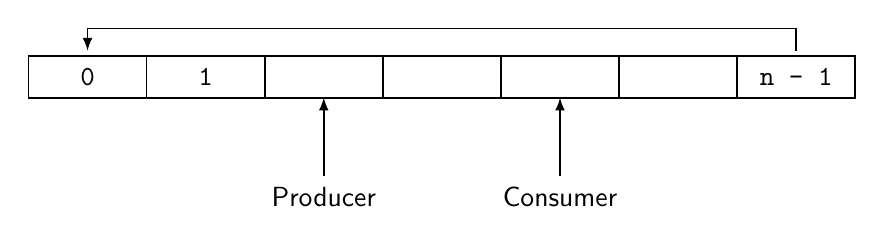
\begin{tikzpicture}[>=latex,font=\ttfamily,
      every node/.style={
        minimum width=1.5cm,
        minimum height=1.5em,
        outer sep=0pt,
        draw=black,
        semithick
      }
    ]
      \node at (0,0) (A) {0};
      \node [anchor=west] at (A.east) (B) {1};
      \node [anchor=west] at (B.east) (C) {};
      \node [anchor=west] at (C.east) (D) {};
      \node [anchor=west] at (D.east) (E) {};
      \node [anchor=west] at (E.east) (F) {};
      \node [anchor=west] at (F.east) (G) {n - 1};
      \draw [->,shorten >=2pt,shorten <=2pt,semithick] (G.north) -- +(0,1em) -| (A);

      \node [below=of C, draw=none] (producer) {\sffamily Producer};
      \draw [->, semithick] (producer) -- (C);

      \node [below=of E, draw=none] (consumer) {\sffamily Consumer};
      \draw [->, semithick] (consumer) -- (E);
    \end{tikzpicture}
    \medskip

    The producer should write to the buffer (if the buffer is not full)

    The consumer should read from the buffer (if the buffer is not empty)
    \medskip

    All consumers share an index and all producers share an index

    \leftspace{}In both cases the index is initially 0 and increases
                 sequentially
  \end{slide}

  \begin{slide}

    \slidetitle{Problem 1: Ensure Producers Never Overwrite Filled Slots}

    \begin{minted}{c}
static uint32_t buffer_size;

void init_semaphores() {
  sem_init(&empty_slots, 0, /* ? */);
}
void producer() {
  while (/* ... */) {
    /* spend time producing data */
    fill_slot();
  }
}
void consumer() {
  while (/* ... */) {
    empty_slot();
    /* spend time consuming data */
  }
}
    \end{minted}

  \end{slide}

  \begin{slide}

    \slidetitle{Use a Semaphore to Track the Number of Empty Slots}

    \begin{minted}{c}
void init_semaphores() {
  sem_init(&empty_slots, 0, buffer_size);
}
void producer() {
  while (/* ... */) {
    /* spend time producing data */
    sem_wait(&empty_slots); /* New */
    fill_slot();
  }
}
void consumer() {
  while (/* ... */) {
    empty_slot();
    sem_post(&empty_slots); /* New */
    /* spend time consuming data */
  }
}
    \end{minted}

    \begin{tikzpicture}[remember picture,
                        overlay,
                        shift={(current page.south west)},
                        show background rectangle]
    \node [align=right, anchor=south east, inner sep=2mm,
           xshift=-2.5em, yshift=2.5em]
          at (\paperwidth, 0)
          {What is our next problem?};
    \end{tikzpicture}

  \end{slide}

  \begin{slide}

    \slidetitle{Problem 2: Ensure Consumers Never Consume Empty Slots}

    \begin{minted}{c}
void init_semaphores() {
  sem_init(&empty_slots, 0, buffer_size);
  sem_init(&filled_slots, 0, /* ? */);
}
void producer() { while (/* ... */) {
  /* spend time producing data */
  sem_wait(&empty_slots);
  fill_slot();
} }
void consumer() { while (/* ... */) {
  empty_slot();
  sem_post(&empty_slots);
  /* spend time consuming data */
} }
    \end{minted}

  \end{slide}

  \begin{slide}

    \slidetitle{Two Semaphores Ensure Proper Order for Producers and Consumers}

    \begin{minted}{c}
void init_semaphores() {
  sem_init(&empty_slots, 0, buffer_size);
  sem_init(&filled_slots, 0, 0);
}
void producer() { while (/* ... */) {
  /* spend time producing data */
  sem_wait(&empty_slots);
  fill_slot();
  sem_post(&filled_slots); /* New */
} }
void consumer() { while (/* ... */) {
  sem_wait(&filled_slots); /* New */
  empty_slot();
  sem_post(&empty_slots);
  /* spend time consuming data */
} }
    \end{minted}

  \end{slide}

  \begin{slide}

    \slidetitle{What Happens If We Initialize Both Semaphore Values to 0?}

    \begin{minted}{c}
void init_semaphores() {
  sem_init(&empty_slots, 0, 0);
  sem_init(&filled_slots, 0, 0);
}
void producer() { while (/* ... */) {
  /* spend time producing data */
  sem_wait(&empty_slots);
  fill_slot();
  sem_post(&filled_slots);
} }
void consumer() { while (/* ... */) {
  sem_wait(&filled_slots);
  empty_slot();
  sem_post(&empty_slots);
  /* spend time consuming data */
} }
    \end{minted}

  \end{slide}

  \begin{slide}

    \slidetitle{We Used Semaphores to Ensure Proper Order}

    Previously we ensured mutual exclusion, now we can ensure order

    \begin{itemize}
      \item Semaphores contain an initial value you choose
      \item You can increment the value using post
      \item You can decrement the value using wait (it blocks if the current
            value is 0)
      \item You still need to be prevent data races
    \end{itemize}

  \end{slide}

\end{document}
